\chapter{自動画像アノテーション}
\section{画像アノテーション}
画像アノテーションとは一般物体認識の要素課題の一つであり,
入力された画像が表す内容に対応するメタデータを付与する技術である.

本研究ではその中でも,予め画像と対応するメタデータを学習をしておくことで,
入力画像に自動でメタデータを付与する自動画像アノテーションを行う.
以下ではこのメタデータをラベルと呼ぶこととする.

\section{一般的な手法}
一般的な自動画像アノテーションの概要を図\ref{fig:abst}に示す.

\begin{figure}[tb]
 \begin{center}
  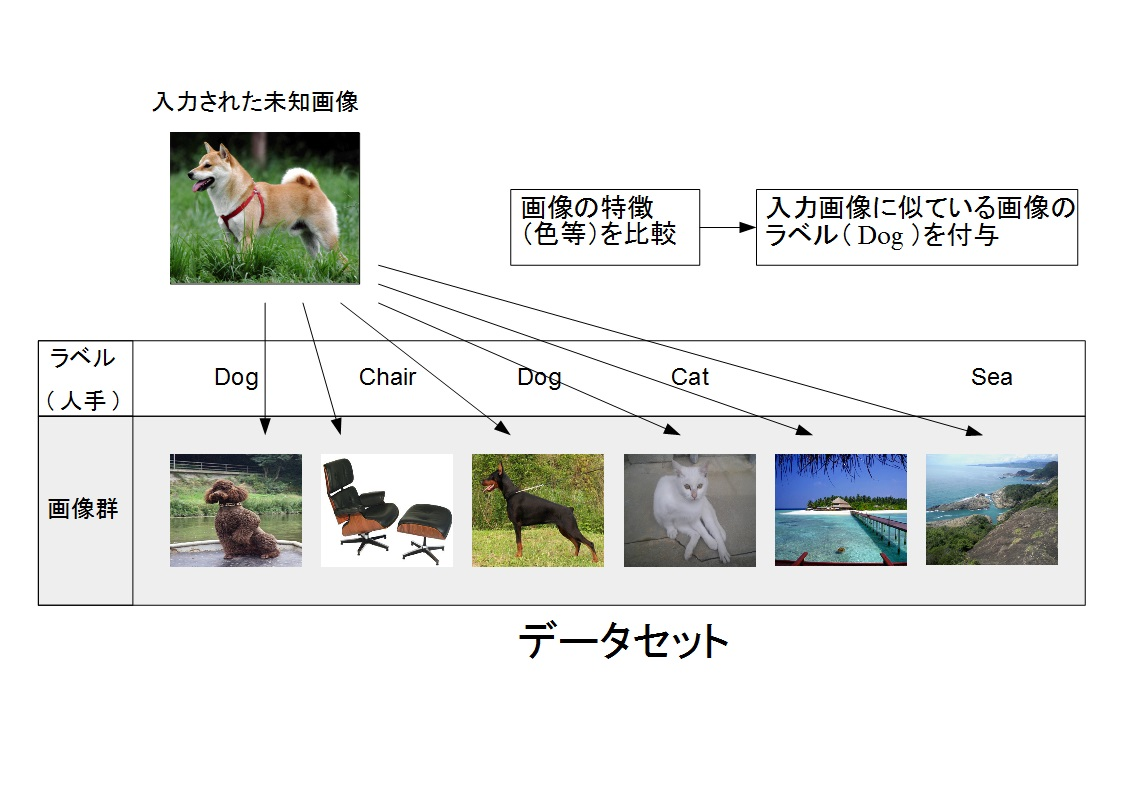
\includegraphics[scale=0.50]{gaiyou.jpg}
 \end{center}
 \caption{一般的な画像アノテーション手法の概要}
 \label{fig:abst}
\end{figure}

まず第一段階として,画像を収集してデータセットを構築し,各画像に人手でラベルをつける.
それらラベルを付けた画像の特徴を統計的に分析することで,ラベルの持つ特徴を学習する.
次に第二段階として,未知の画像を入力し,その画像特徴と類似する画像群が共通して持つラベルを見つけ,
入力画像にそのラベルを付与する.

本稿では,画像の分類手法に工夫をこらし,入力画像に対するラベル付与の精度を高めるための実験を行った.
自動画像アノテーションの分野における主な研究としてはこの他にも,
画像の収集や画像に対するラベル付与を自動化することで,データセットの構築にかける時間と労力を減らす手法などが提案されている.

\chapter{関連研究}
\label{sec:related}
前節でラベル付与の自動化・高精度化の手法が研究されていると述べた.
それらの研究の中でも近年頻繁に研究されているものが,画像のブロブ化である.
ブロブ化は各画像を複数の領域に分割し,隣接する領域との特徴の差異を見ることで画像全体を分解することで行う.
これによって得られたブロブは,画像に写っている物体ごとに分割されている可能性が高いので,
注目しているブロブ以外の物体の有無に左右されることなく,そのブロブに対する精確なラベル付与が可能となる.
このブロブ化をデータセット内の全ての画像に施すことで,高精度の画像アノテーションを実現する.

Duygulu\cite{duygulu}らやJeon\cite{jeon}らは,すべての画像はブロブ(画像内の物体の塊)に単語を割り当てることで
内容物を記述することができるという前提で研究を行った.
JeonはDuyguluらの研究を元に,まずブロブと単語の同時分布を予習するためにCMRM(Cross-Media Relevance Model)を開発し,
更にそのモデルを改良した3つのモデルを開発した.
これらは画像を収集する際に自動で画像アノテーションを行う確率的生成モデルである.
その結果,Duyguluらが論文で公開した確率的生成モデルの画像アノテーションの平均精度0.20に比べ,
ほぼ倍の0.41という平均精度を示し,再現率についてもはるかによい結果となった.

またこれらの研究とは別のアプローチで画像アノテーションの精度向上を目指した研究がある.
渡邉ら\cite{watanabe}は,大規模Web画像データベースと
類似画像検索技術を用いた自動画像アノテーションシステムを実装した.
このシステムは,与えられた画像をクエリとして類似画像検索を行い,
検索結果の画像に付随するテキスト中の単語を確率的指標により評価することで,
特別な事前学習なしに画像を意味付けるキーワードを推定可能であることを示した.
このシステムを用いて5カテゴリ30概念の画像に対するアノテーションを行った結果,
10位内正解率がカテゴリ平均で43~75\%,全概念の平均で約59.1\%であった.

\chapter{類似画像検索とテキスト検索を用いた自動画像アノテーション}
\label{sec:way}
\section{提案手法の概要}
本研究で提案する自動画像アノテーション手法の概要を説明する.(図\ref{fig:way}参照).

\begin{figure}[tb]
 \begin{center}
  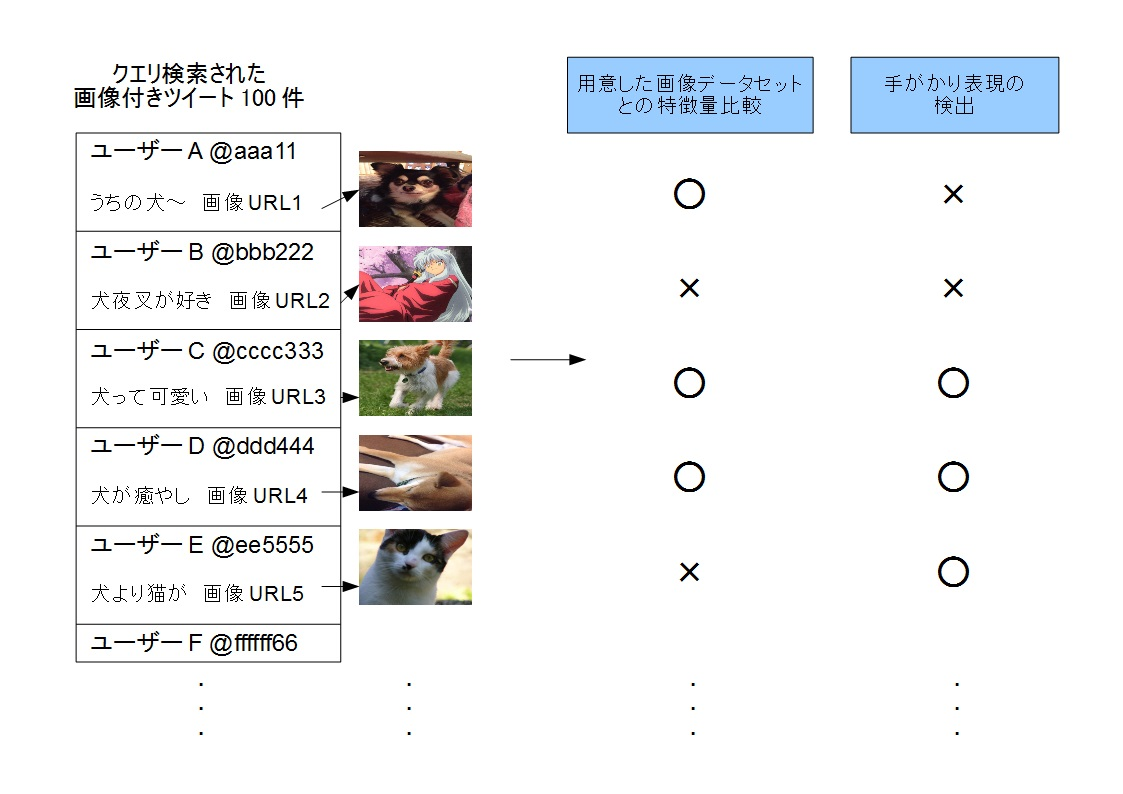
\includegraphics[scale=0.50]{way.jpg}
 \end{center}
 \caption{提案手法の概要}
 \label{fig:way}
\end{figure}

本手法における処理は,Webから得られた画像と周辺テキストを収集する前処理と,
類似画像検索とテキスト検索を用いて得られた画像を分類する処理に分けられる.

前処理においては,TwitterAPIを利用し,物体名をクエリに指定して検索を行い,得られたツイートを収集する.
収集したツイートから上位100件を選び,それらのツイートに付随するURLからTwitterの公式アップローダにアップロードされた画像をそれぞれ取得する.
%\item 収集したツイートから上位100件を選び,クエリで指定した物体を表しているかどうかを人手で判別する.

画像分類処理においては,まず,ユーザが前処理でクエリとして選んだ物体を表す参考画像を数枚収集し,
その画像を一枚ずつクエリとして,100枚の画像に対して類似画像検索を行う.
参考画像とは,クエリを正しく表していると実験者が判断し,類似画像検索の比較元とする画像である.
類似画像検索は,画像の持つ色や形状などの特徴による検索であり,
この結果,参考画像と見た目の類似した画像が得られる.

また,収集したツイート本文にも手がかり表現を用いてテキスト検索を行う.
この手がかり表現とは,付随する画像が何を表しているかの手がかりとなる表現のことで,
ツイート中からその表現を検索することで,そのツイートに付随する画像がクエリを正しく表現しているか否かの分類が行える.

この二手法を組み合わせ,クエリ単体の自動画像アノテーションを実現している.

以下では,ツイート収集と,類似画像検索,テキスト検索について詳細に説明する.

\section{ツイートの収集}
TwitterAPI1.1の機能を使い,検索したい画像の名称をクエリとし,Twitterからツイートを検索する.
この際,オプションとして" -RT filter:images"をクエリに含めることで,ある程度収集するツイートを選別する.
" -RT"は重複したツイートを取得することを避けるために,
" filter:images"はTwitterの公式アップローダにアップロードされた画像のみを参照するために使用する.

\section{類似画像検索}
本手法では,各色が画像中に何ピクセルあるかを数えた色ヒストグラムを特徴量として比較を行い,
その結果から類似画像の検索を行う.
そのため,収集したツイートのクエリを正しく表している参考画像を,ツイートに付随する画像とは別に10枚収集する.

まず,収集した画像110枚を全てJPEG形式に変換する.
これは色ヒストグラムを算出する際に,全ての画像において画素の記述方法を統一するためである.
次に,収集した100枚の画像と10枚の参考画像の色ヒストグラムを算出し,それぞれファイルに保存する.
ただし,色ヒストグラムは各色8ビットをそのままで計算すると16,777,216次元ベクトルとなってしまうため,
各色を4分割した64色に減色した上で算出する.

各画像の色ヒストグラムデータを作成したら,各参考画像をクエリとして,
Histogram Intersectionで各画像に対する類似度を10枚分算出する.
それら10個の類似度の中で最も高い値をクエリ類似度として,設定した閾値を超えた画像を,クエリを表している画像として分類する.
%%%%%%%%%%閾値が明確に決められない場合にROCカーブを描いて性能を比較する場合も%%%%%%%%%%%%
%%閾値を 0 から1まで 0.01 ずつ大きくしていき,それぞれの閾値において類似画像検索の適合率と再現率を求める.%%
\section{テキスト検索}
収集してきたツイートの本文から手がかり表現を見つけ,そのツイートの持つ画像を分類する.
このとき,"本物","写真","いる","撮"のいずれかの文字列を含んでおり,
かつ"描"の文字を含まないツイートの持つ画像は,クエリとして選んだ物体を表していると判断する.

\chapter{評価実験}
\label{sec:experiment}
\section{データセット}
本稿では,Twitterに投稿された画像付きツイートを収集し,データとして用いた.
データの収集は2015年1月8日に,"犬 -RT filter:images"をクエリとしてツイートを検索し,
その結果として得られたツイートの上位100件を収集した.
そして,得られたツイートに付随する画像を1つずつ収集し,人手で犬を表しているか判別した.
これら100件のツイートと100枚の画像をデータセットとした.

\section{評価方法}
本手法による結果と人手で画像を分類した結果とを比較し,画像分類精度を評価する.

まず,各画像に対し,人手で犬を表している画像かどうかを判定したものを正解データとする.
データセットの画像100枚の内,犬の画像であると判断した画像は46枚であった.

これに対し,各画像の色ヒストグラムデータを作成し,参考画像と比較してクエリ類似度を算出する.
求めたクエリ類似度が設定した閾値を上回る画像を,犬を表している画像として分類する.
値の設定は暫定的に0.6とした.

また,収集したツイートに対してテキスト検索を行い,条件を満たしたツイートに付随する画像を犬を表している画像として分類する.

この二手法の分類結果を組み合わせた画像の分類も行う.
どちらか片方の分類手法で犬の画像であると判断された画像は,
もう一方で犬の画像ではないと判断された画像でも犬の画像であるとした.

類似画像検索,テキスト検索,二手法の組み合わせにおいて,分類した画像の適合率と再現率を求める.
ここで,適合率は類似画像検索の分類結果に含まれる正解データの割合であり,再現率は人手で判定した犬を表す画像のうち
実際に分類できていた正解データ画像の割合である.
さらに,求めた適合率および再現率から F 値を算出する.
F 値($F\verb|-|measure$)は適合率($precision$)と再現率($recall$)の調和平均であり,次式で求める.

\begin{eqnarray}
F\verb|-|measure = \frac{2・precision・recall}{precision+recall}
\end{eqnarray}

類似画像検索,テキスト検索,二手法の組み合わせによる画像分類の結果を表\ref{tab:result}に示す.

\begin{table}[tb]
\begin{center}
\caption{各手法による適合率,再現率,F値}
\label{tab:result}
\begin{tabular}{|l|r|r|r|}\hline
& 適合率& 再現率& F値\\ \hline \hline
類似画像検索(1)& 0.627& 0.804& 0.705 \\ \hline
テキスト検索(2)& 0.833& 0.109& 0.192 \\ \hline
二手法の組み合わせ(1+2)& 0.633& 0.826& 0.717 \\ \hline
\end{tabular}
\end{center}
\end{table}

\section{類似画像検索による画像分類精度評価}
画像の色ヒストグラム比較による分類では,適合率が約0.627,再現率が約0.804,F値が約0.705となった.
この値は仮に閾値を0.6とした場合であるため,閾値が適切かどうかを確かめる実験もすべきである.

\section{テキスト検索による画像分類精度評価}
ツイート文のテキスト検索による分類では,適合率が約0.833,再現率が約0.109,F値が約0.192と,再現率の値が低かった.
これは,条件を厳し目にし,類似画像検索での正解データの取りこぼしをなくせるように設定したため,
正解数に対し極小数の画像のみを正解とみなしたからである.
また,ツイートにおけるテキストの量が少量であるため,テキスト検索により多くの正解データを当てることは困難である.

\section{二手法の組み合わせによる画像分類精度評価}
両手法を組み合わせた分類結果では,適合率が約0.633,再現率が約0.826,F値が約0.717となった.
精度・再現率・F値の全てにおいて類似画像検索のみの実験結果より向上している.
2つの手法の結果から正解データを多く網羅することができたため,全体的な精度が向上したとみられる.

今回の実験では正解データ数が極端に少ないため,精度の信頼性がなく,
また有用な表現も見つけることが出来なかった.
よって,狐以外のクエリでも実験を行う,参考にする画像の量を変動させ結果の推移を見る,
類似度の閾値を調整するなどして,有効な実験の条件を検討していく予定である.

